\documentclass{article}
\usepackage{graphicx}
\usepackage{subcaption}
\usepackage{textcomp}

% to make table of contents clickable
\usepackage{hyperref}
\hypersetup{
}

\author{CD}
\title{DD}

\begin{document}

\thispagestyle{empty} % to hide pagenum
\begin{center}

	\vspace{3cm}

	\large $\bf Software$ $\bf Engineering$ $\bf 2$

  
\includegraphics[width=\linewidth]{../RASD/images/polimi-logo.png}
  \vspace{2cm}
  

  \Huge $\bf SafeStreets$


	\huge $\bf Design$  $\bf Document$

	\vspace{1cm}

  Authors:
	\vspace{1cm}
	\begin{tabular}{r|l}
		 Federico Cazzola & \large mat 945835\\
		 Francesco Dotti & \large mat 945232\\
	\end{tabular}

	\vspace{1cm}

  Professor: Di Nitto Elisabetta
	
	\vspace{3cm}
  \normalsize Academic Year 2019-2020

	\vspace{2mm}
	\small Version 1.0

\end{center}

\newpage

\thispagestyle{empty} % to hide pagenum
\tableofcontents

\newpage
  
\section{Introduction}
\subsection{Purpose}
The purpose of this document is to describe how the system will be built, giving specific and technical details about architectural and design decisions. Also implementation, integration and testing plans will be discussed.
In particular the document presents:
\begin{itemize}
	\item The SafeStreet System architecture (its parts and how they interact)
	\item The runtime behavior
	\item The design patterns
	\item User Interfaces
	\item Implementation, integration and testing plans 
\end{itemize}

\subsection{Scope}
The scope of the Safestreets project, as already specified in the RASD, is to give the user the possibility to report traffic violation, in particular, parking violation (eg. parking in a spot reserved for disabled people, parking in an helicopter pitch, parking on the sidewalk).\\
The system will allow the users to select the type of violation leading to differt amount of ticket value.\\
The system will help the authorities to identify more infractions and therefore to issue more tickets which should increase the attention and respect of the citizens regarding the traffic rules.\\
Furthermore, thanks to the increased number of tickets, the municipality will have more money to invest in the community. This extra money could be used to do some interventions following the suggestions provided by SafeStreets.

\subsection{Definitions, Acronyms, Abbreviations}
\subsubsection{Definitions}
\begin{itemize}
\item \textbf{Mine}: to process data for obtaining new data
\item \textbf{Violation}: an infringement of the rules
\item \textbf{Unsafe}: area area where often happen violation and accident
\item \textbf{Report Open}: a report with no traffic warden assigned
\end{itemize}

\subsubsection{Acronyms}
\begin{itemize}
	\item \textbf{RASD}: Requirements Analysis and Specifications Document  
	\item \textbf{DD}: Design Document
	\item \textbf{FOSS}: Free and Open Source Software
	\item \textbf{S2B}: Software to Be
	\item \textbf{API}: Application Programming Interface
	\item \textbf{ALPR}: Automated License Plate Recognition
	\item \textbf{JS}: JavaScript
	\item \textbf{JWT}: JSON Web Tokens
	\item \textbf{FCM}: Firebase Cloud Messaging
	\item \textbf{REST}: REpresentational State Transfer
	\item \textbf{DBMS}: Database Management System
	\item \textbf{SDK}: Software Development Kit
	\item \textbf{UX}: User eXperience
\end{itemize}

\subsubsection{Abbreviations}
% \begin{itemize}
% \end{itemize}

\subsection{Revision history}
\begin{itemize}
	\item Version 1.0 | First Release
\end{itemize}

\subsection{Reference Documents}
\begin{itemize}
	\item Specification document: “SafeStreets Mandatory Project Assignment” 	
	\item \href{https://www.uml-diagrams.org}{UML diagrams}
	\item IEEE Standard for Information Technology—Systems Design—Software Design Descriptions (IEEE Std 1016TM-2009)
\end{itemize}

\subsection{Document Structure}
\begin{itemize}
	\item Chapter 1 is the introduction.
	\item Chapter 2 provides details about the system architecture, its components and how they interact.
	\item Chapter 3 describes the UX and shows the user interface providing mockups.
	\item Chapter 4 describes how the requirements ( defined in the RASD ) are mapped to the design elements defined in this document.
	\item Chapter 5 presents the implementation, integration and test plan. It shows how the different components of the application are integrated with each other and how they react. Also the testing strategies are described and the risks in the application are analyzed.
	\item Chapter 6 shows the effort spent by each group member
\end{itemize}

\newpage

\section{Architectural design}
\subsection{Overview: High-level components and their interaction}
\label{sec:Overview}
The application will be developed with three logic software layers: 
\begin{itemize}
	\item Presentation (P) manages the user interaction with the system 
	\item Application (A) handles the business logic of the application and its functionalities 
	\item Data access (D) manages the information with access to the database
\end{itemize}
These layers are thought to be divided on three different hardware tiers (a machine or a group of machines), so that any logic layer has, in principle, its own dedicated hardware (three-tier architecture).\\
This architecture should give the system more scalability and flexibility as the server side is split into two nodes.\\
The second tier must contain only the business logic to physically separate clients and data to guarantee more safety in accessing to data since the system deals with sensitive data. \\
The following image shows an high-level view of the architecture of the system using the ArchiMate modeling language.\\
\\
\begin{figure}[ht]
\centering
	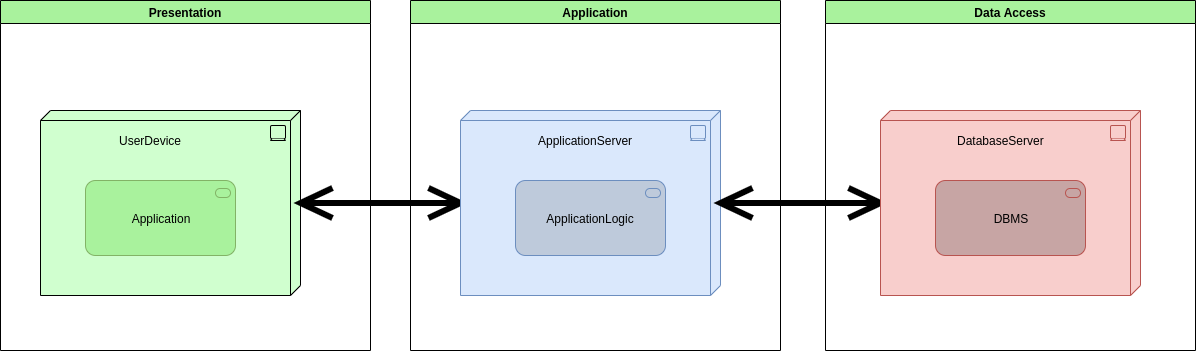
\includegraphics[width=1.0\textwidth]{images/tier-structure.png}
	\caption{SafeStreets 3-tier architecture}
	\label{fig:tier-structure}
\end{figure}

\newpage

\subsection{Component view}

In the following diagram only the application server is analyzed in detail

\begin{figure}[!htb]
\centering
	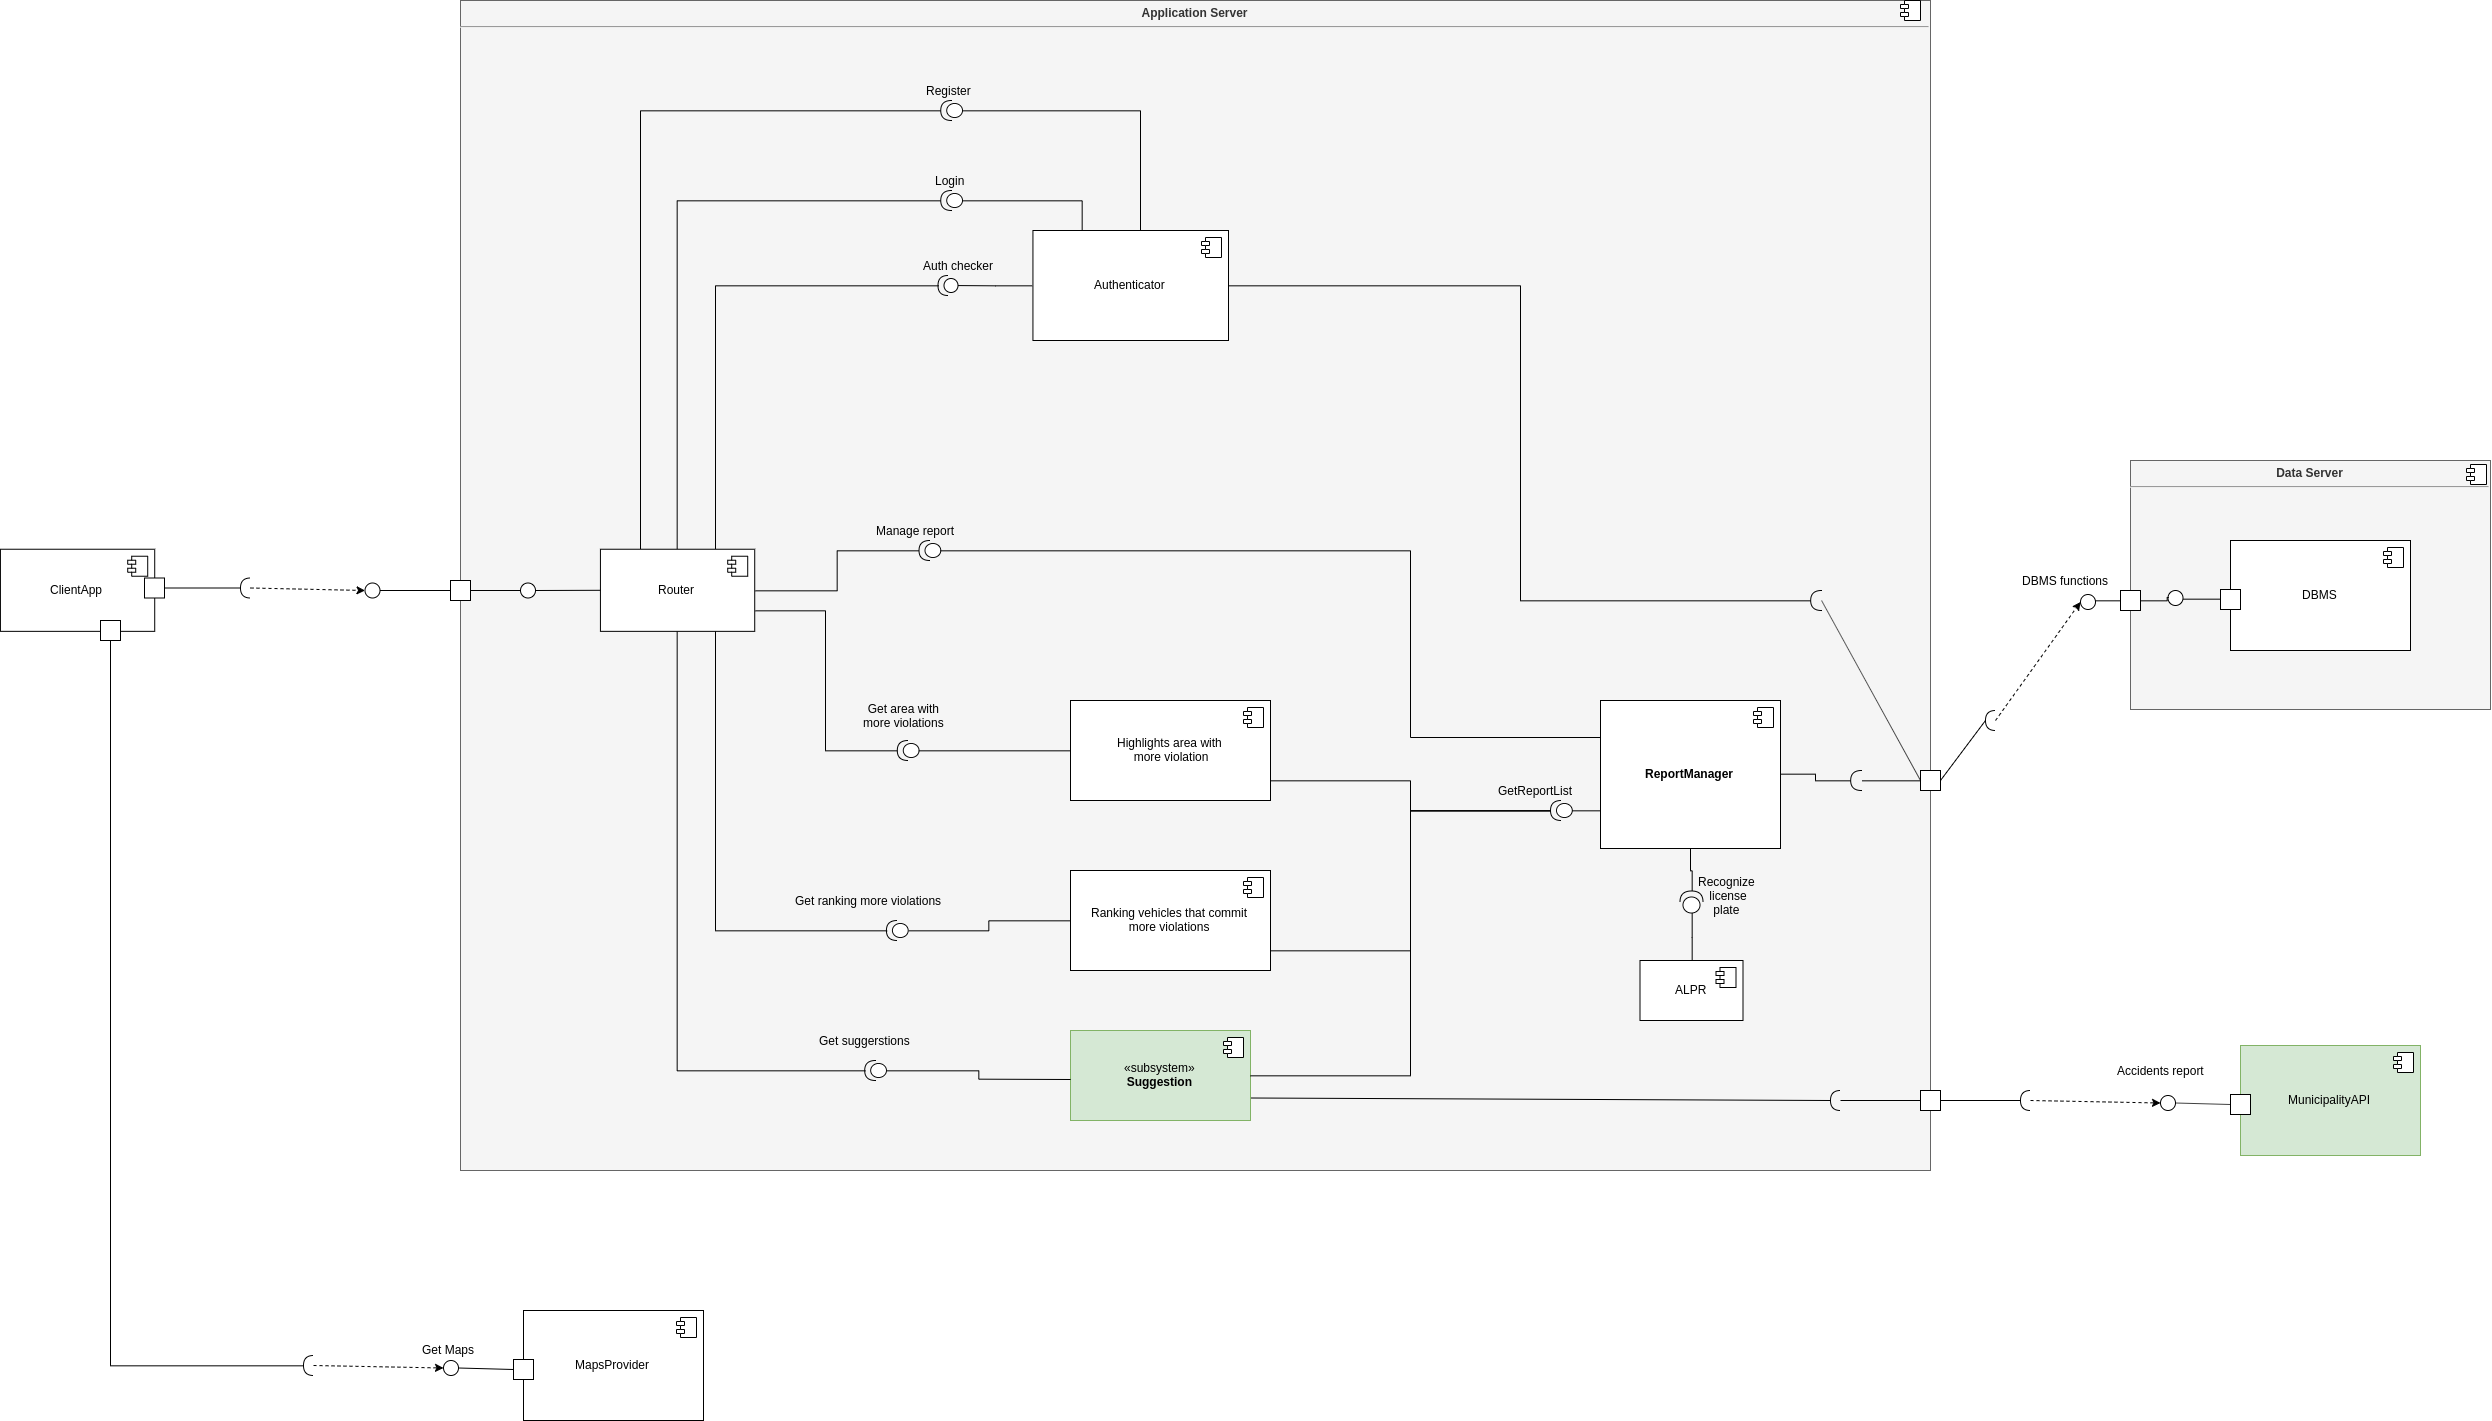
\includegraphics[width=1.0\textwidth]{images/components-diagram.png}
	\caption{Component diagram}
	\label{fig:component-diagram}
\end{figure}

Here are described more in detail all the components and interfaces that
the application server uses to offer its functionalities.
\begin{itemize}
	\item \textbf{Router}: Manages all the request coming from the clients, forwarding them in the appropriate component for the specific request. 
	It also interacts with the \textit{Authenticator component} to check if a request comes from an authenticated user and then denies or forwards the request according to the user permissions.
	\item \textbf{Authenticator}: Manages the sign up and login requests and checks if a request comes from an authenticated user.
	\item \textbf{ReportManager}: Manages all the requests inerent to reports (e.g. get list of report, send new report) and is responsible to check if the new reports are consistent. Also collects reports form the database to pass them to other components.
	\item \textbf{Area-Highlighter}: Elaborates the reports to find in which area more violations are committed.
	\item \textbf{RankingManager}: Elaborates the valid reports to create a ranking of the vehicles that committed more violations.
	\item \textbf{NotificationManager}: Manages all the subscriptions for notification made by the client's app when a traffic warden log in and send the notification to them when a new report is added.
	\item \textbf{ALPR}: Elaborates the picture of the violation to extract the license plate. This component is designed to be separate by the others so that if after deployment it will became overload it could be deployed on a different server.
	\item \textbf{SuggestionSubsystem}: More in detail:
		\\
\begin{figure}[!htb]
\centering
	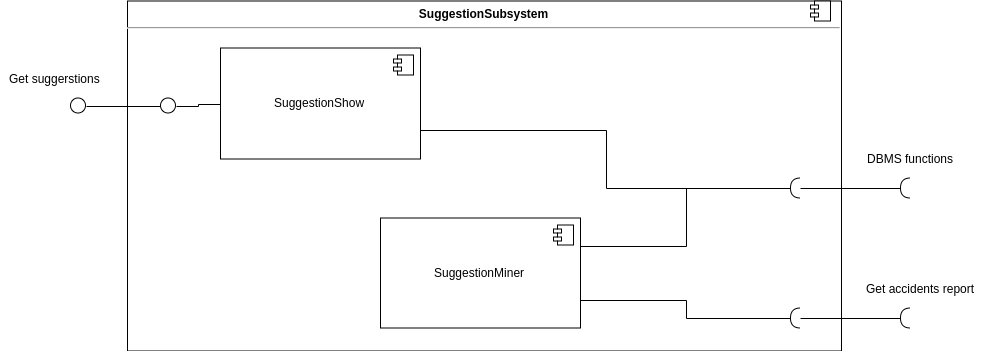
\includegraphics[width=1.0\textwidth]{images/SuggestionSubsystem-components-diagram.png}
	\caption{Component diagram suggestion subsystem}
	\label{fig:component-suggestion-subsystem}
\end{figure}
\begin{itemize}
	\item \textbf{SuggestionDisplayer}: Sends the list of the suggestions
	\item \textbf{SuggestionMiner}: Gets data from Muncipality's servers and from Safestreets' database and elaborates the suggestions for possible interventions
\end{itemize}
\end{itemize}

\newpage

\subsection{Deployment view}
\label{sec:Deployment}
The following diagram models the physical deployment of artifacts (software components) on nodes (hardware components).
External services like the Map Provider are not included.
\begin{figure}[!htb]
\centering
	\includegraphics[width=1.0\textwidth]{images/deployment_diagram.png}
	\caption{Deployment diagram}
	\label{fig:deployment-diagram}
\end{figure}

	
\begin{itemize}
	\item \textbf{Tier 1} \\
		Users can access the SafeStreets service using the mobile application available for Android and iOS devices or using the web app (compatible with any modern browser).
		The web app will communicate directly with the application server using RESTful API,
		exactly like the apps for iOS and Android.
	\item \textbf{Tier 2} \\ 
		The same server machine (for budget reasons)  will contain all the components handling the business and the web logic.
		The application server handles all the requests coming from the users applications. 
		The web server is just there to make possible to get the web app from a website. 
	\item \textbf{Tier 3} \\
		The database machine will run MySQL server (a relational database management system). On this machine will be stored all the persistent data.
\end{itemize}
		\small Note1: The webserver will not be mentioned in the next sections. It would be like including the AppStore or GooglePlay. However it has to be deployed.\\
		\small Note2: The ClientAPP will work in same way on every platform.

\newpage
\subsection{Runtime view}
\label{sec:Runtime}
 In this section are shown the sequence diagrams of some features. They are useful to clarify the runtime behaviour of the components involved for each functionality.\\
 In order to keep the diagrams more readable the parameters of the method invoked are not shown.
The numbers present in some responses refer to HTTP response status codes:
\begin{itemize}
	\item \textbf{201 Created}: The request has been fulfilled, resulting in the creation of a new resource.
	\item \textbf{400 Bad Request}: The server cannot or will not process the request due to an apparent client error (e.g., malformed request syntax, size too large, invalid request message framing, or deceptive request routing).
	\item \textbf{401 Unauthorized}: The user does not have valid authentication credentials for the target resource.
	\item \textbf{409 Conflict}: Indicates that the request could not be processed because of conflict in the current state of the resource. 
\end{itemize}


\newpage
\subsubsection{Report Violation}
\begin{figure}[!htb]
\centering
	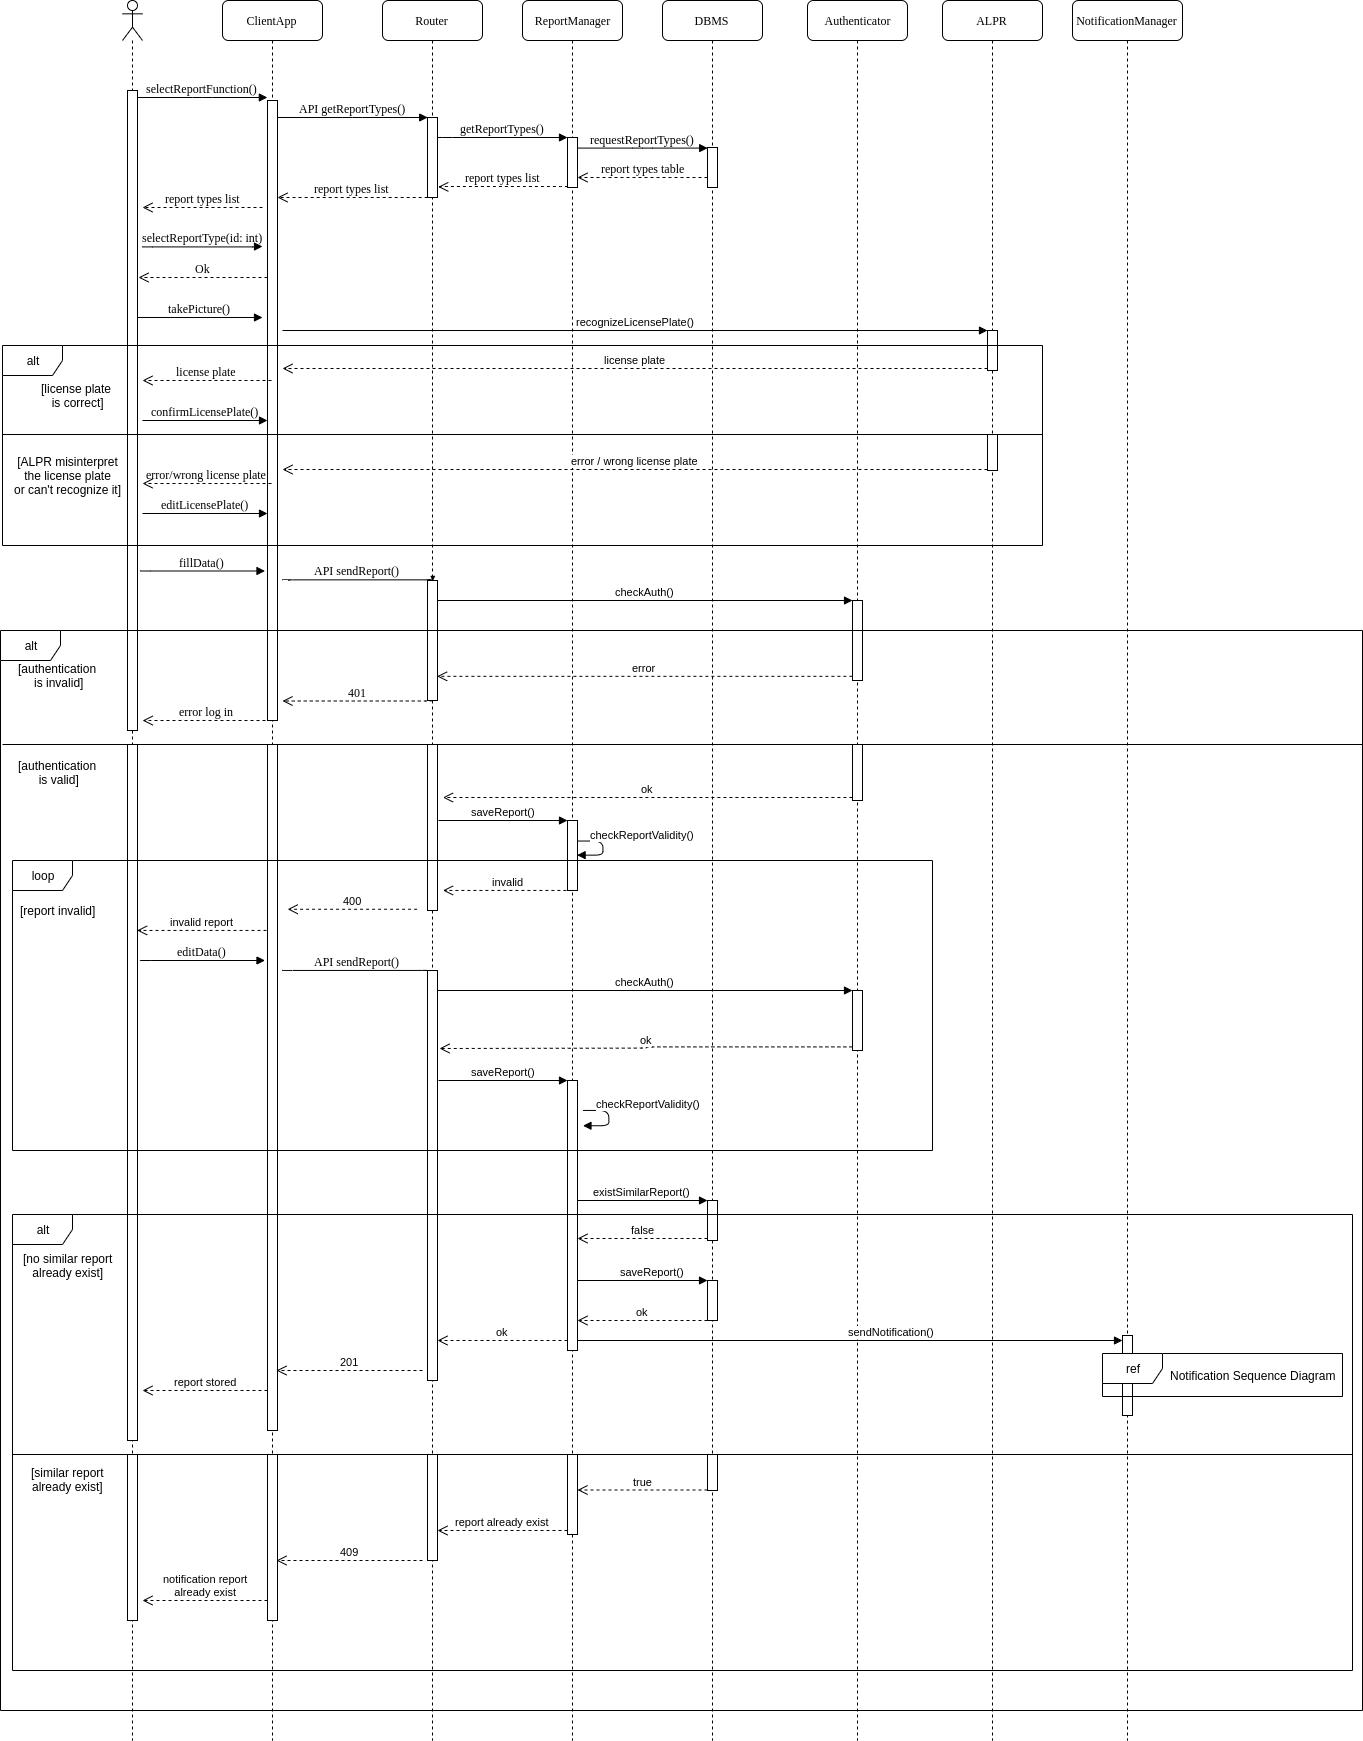
\includegraphics[width=1.0\textwidth]{images/report-violation-sequence.png}
	\caption{Report violation sequence diagram}
	\label{fig:report-violation-sequence-diagram}
\end{figure}
\subsubsection{Traffic warden receives notification}
\label{sec:notification}
\begin{figure}[!htb]
\centering
	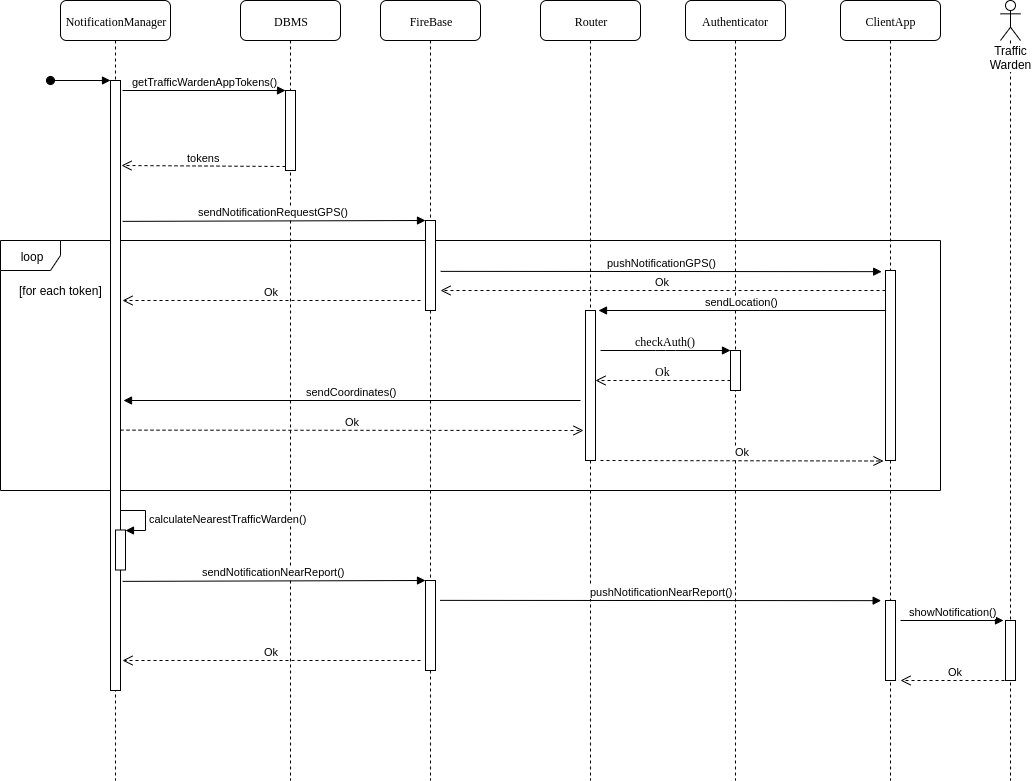
\includegraphics[width=1.0\textwidth]{images/notification-sequence.png}
	\caption{Traffic warden gets notification sequence diagram}
	\label{fig:notifaction-sequence}
\end{figure}
Firebase Cloud Messaging (FCM) is a cross-platform messaging solution that lets you reliably deliver messages at no cost.
Using FCM, we can notify a traffic warden client app that a new report to take on is available.

\newpage
\subsubsection{Traffic warden takes on report}
\label{sec:traffic-warden}
\begin{figure}[!htb]
\centering
	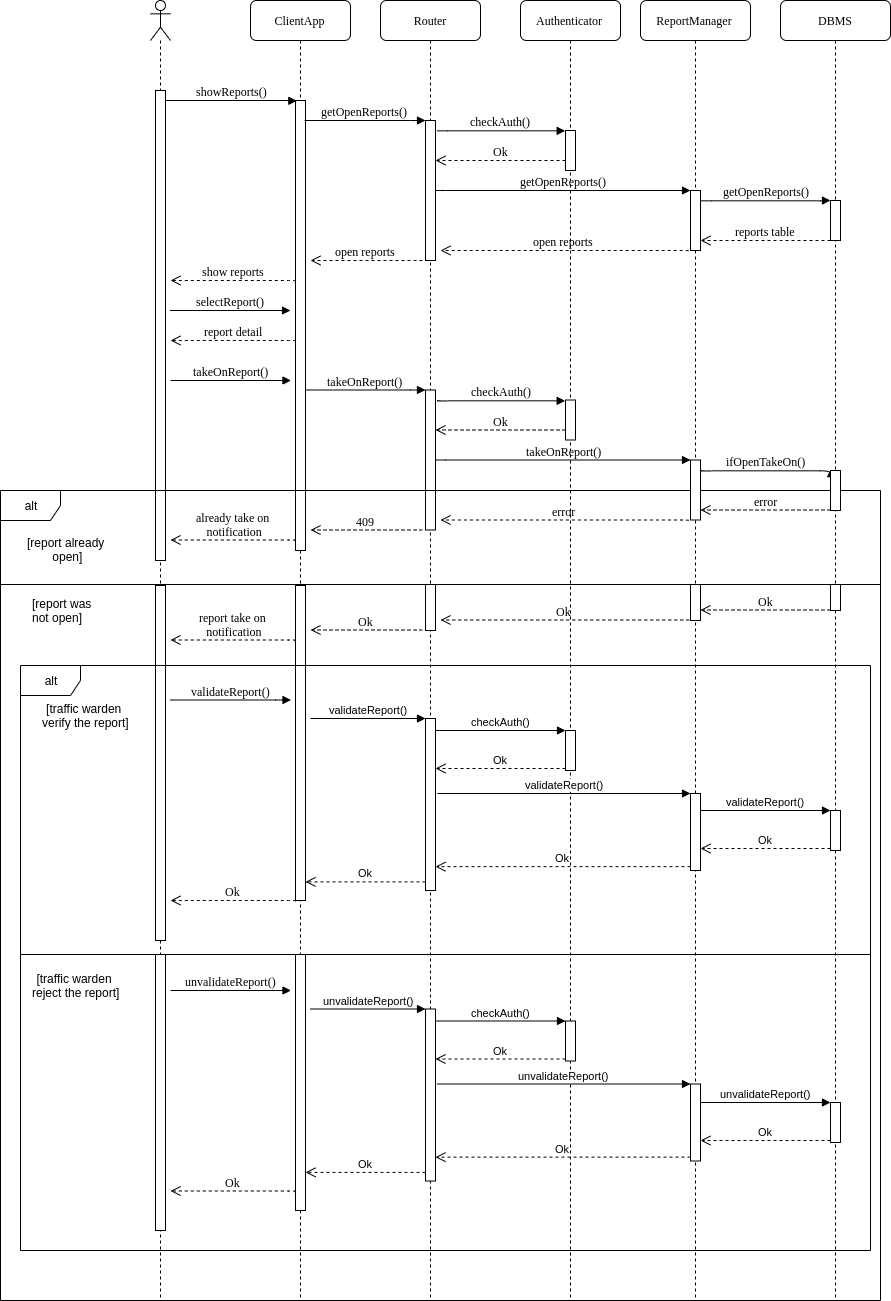
\includegraphics[width=1.0\textwidth]{images/traffic-warden-report.png}
	\caption{Traffic warden takes on report sequence diagram}
	\label{fig:traffic-warden-sequence}
\end{figure}

\newpage
\subsubsection{Login}
\begin{figure}[!htb]
\centering
	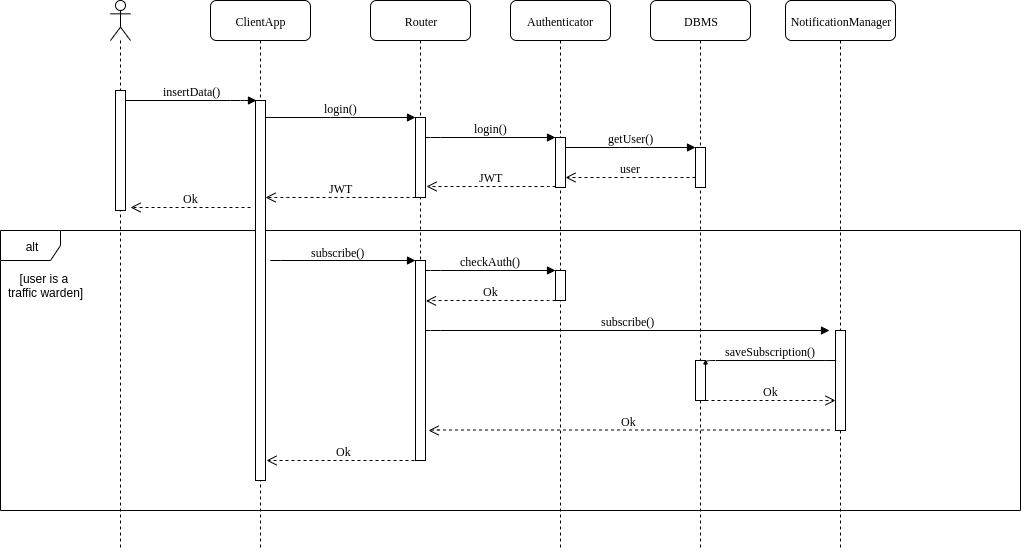
\includegraphics[width=1.0\textwidth]{images/login-sequence-diagram.png}
	\caption{Login sequence diagram}
	\label{fig:login-sequence-diagram}
\end{figure}
Standard RESTful login process exploiting JWTs. \\
This diagram also shows the differences in the login process between a standard user and a traffic warden. The latter must also receive notifications so the NotificationManager is required.

\newpage
\subsubsection{Cross data to suggest possbile interventions}
\begin{figure}[!htb]
\centering
	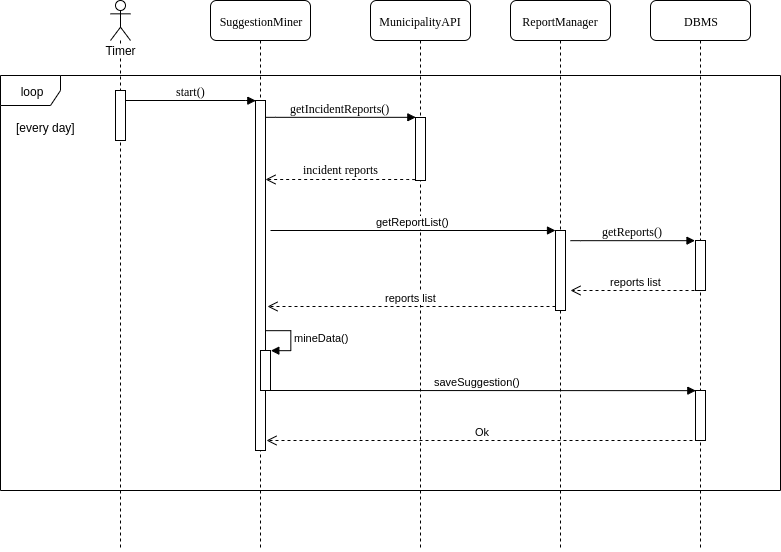
\includegraphics[width=1.0\textwidth]{images/miner-sequence-diagram.png}
	\caption{Suggestions sequence diagram}
	\label{fig:miner-sequence-diagram}
\end{figure}

The diagram shows how there are no human actors involved. This is an automated process triggered by a timer (runs once every day). \\
The data needed by the SuggestionMiner are fetched from the Municipality Server and from the SafeStreets DBMS. The updated suggestions list is then stored on the database.
\newpage
\subsubsection{Visualize critical areas on the map}
\begin{figure}[!htb]
\centering
	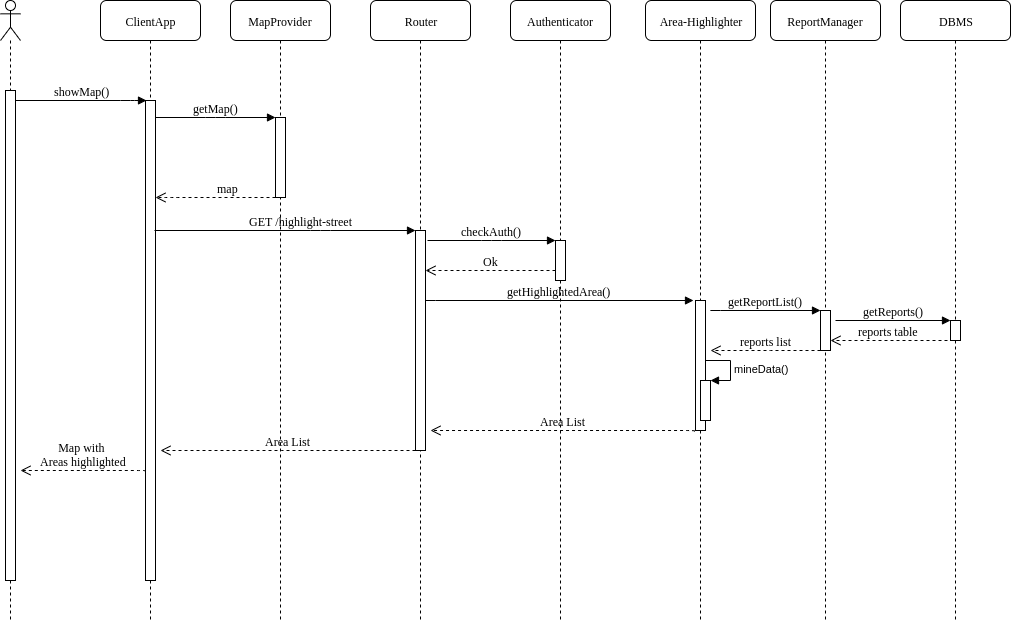
\includegraphics[width=1.0\textwidth]{images/area-highlight-sequence.png}
	\caption{Areas sequence diagram}
	\label{fig:area-highlight-sequence}
\end{figure}

\newpage
\subsubsection{Visualize the ranking of vehicles that committed more violations}
\begin{figure}[!htb]
\centering
	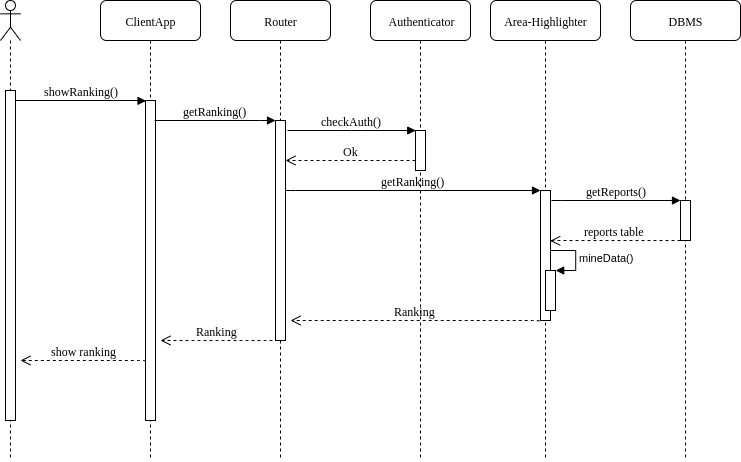
\includegraphics[width=1.0\textwidth]{images/ranking-sequence.png}
	\caption{Vehicles ranking sequence diagram}
	\label{fig:ranking-sequence}
\end{figure}

\newpage
\subsubsection{Visualize suggestions for possible interventions}
\begin{figure}[!htb]
\centering
	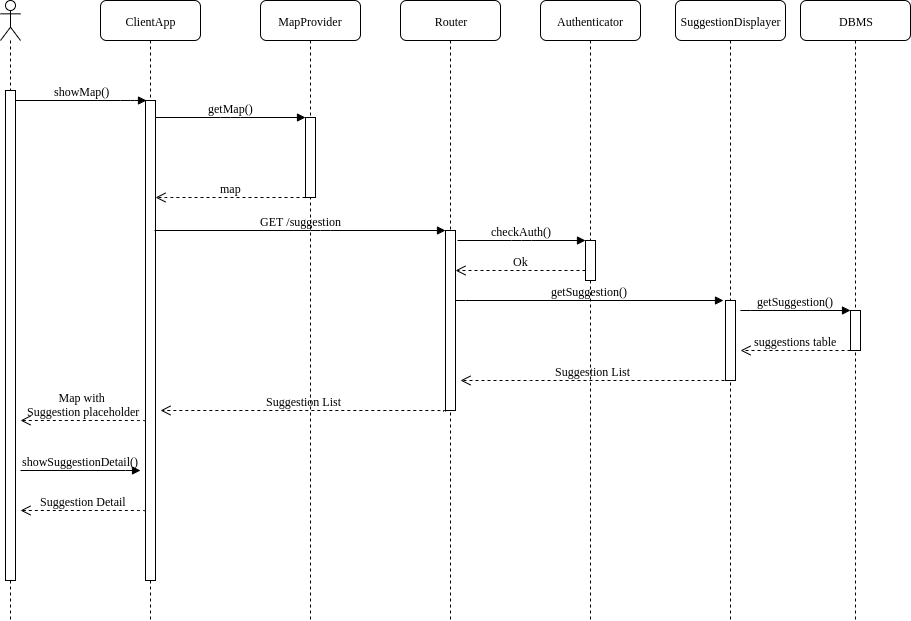
\includegraphics[width=1.0\textwidth]{images/visualize-suggestion-sequence.png}
	\caption{Suggestions sequence diagram}
	\label{fig:visualize-suggestion-sequence}
\end{figure}

\clearpage
\subsection{Database View}
It is also important to describe how data are stored.
Here we report a simple Entity-Relationship diagram. 
This model defines the structure which will be implemented in the MySQL database.\\ \\ \\
\begin{figure}[!htb]
	\centering
		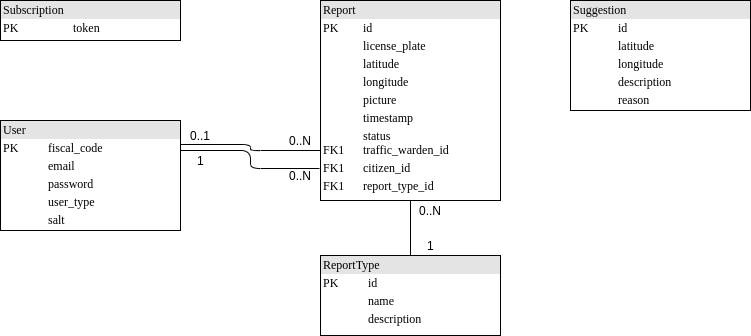
\includegraphics[width=1.0\textwidth]{images/database-diagram.png}
		\caption{Database ER diagram}
	\end{figure}

\newpage
\subsection{Component interfaces}
Here are provided details on methods on interfaces previously indentified. Labels in messages used in the runtime view sequence diagrams must be consistent with the interfaces of components.
\\
This viewpoint consists of a set of interface specifications for each entity.

\begin{itemize}
	\item \textbf{Router}:
		\begin{itemize}
			\item \textbf{GET /report/type}:
				Get all the reports' types
				\begin{itemize}
					\item \textbf{Parameters}:
						\begin{itemize}
							\item none
						\end{itemize}
					\item \textbf{Return}:
						\begin{itemize}
							\item reportType: \textlangle{}ReportType\textrangle{}
						\end{itemize}
				\end{itemize}
			\item \textbf{POST /report}:
				Post a new report
				\begin{itemize}
					\item \textbf{Parameters}:
						\begin{itemize}
							\item JWT
							\item report: Report
						\end{itemize}
					\item \textbf{Return}:
						\begin{itemize}
							\item 201: created
							\item 401: report invalid
							\item 409: report already exist
						\end{itemize}
				\end{itemize}
			\item \textbf{POST /login}:
				Log in
				\begin{itemize}
					\item \textbf{Parameters}:
						\begin{itemize}
							\item email: String
							\item password: String
						\end{itemize}
					\item \textbf{Return}:
						\begin{itemize}
							\item JWT
						\end{itemize}
				\end{itemize}
			\item \textbf{POST /subscribe}:
				Subscribe to recive notification for new report (only user defined as traffic warden can access)
				\begin{itemize}
					\item \textbf{Parameters}:
						\begin{itemize}
							\item JWT
							\item token: String \textit{token used for firebase}
						\end{itemize}
					\item \textbf{Return}:
						\begin{itemize}
							\item 200
						\end{itemize}
				\end{itemize}
			\item \textbf{GET /highlight-area}:
				Get the area with more violation
				\begin{itemize}
					\item \textbf{Parameters}:
						\begin{itemize}
							\item JWT
							\item filter: List\textlangle{}ReportType\textrangle{}
							\item from: Date \textit{analyze data only starting from this date}
							\item to: Date \textit{analyze data only until this date}
						\end{itemize}
					\item \textbf{Return}:
						\begin{itemize}
							\item areas: List\textlangle{}Area\textrangle{}
						\end{itemize}
				\end{itemize}
			\item \textbf{GET /ranking}:
				Get the ranking of the license plate that committed more violation
				\begin{itemize}
					\item \textbf{Parameters}:
						\begin{itemize}
							\item JWT
							\item filter: List\textlangle{}ReportType\textrangle{}
							\item from: Date \textit{analyze data only starting from this date}
							\item to: Date \textit{analyze data only until this date}
						\end{itemize}
					\item \textbf{Return}:
						\begin{itemize}
							\item ranking: List\textlangle{}String\textrangle{} \textit{ordered list of license plate}
						\end{itemize}
				\end{itemize}
			\item \textbf{GET /suggestion}:
				Get the suggestions (only user defined as municipality can access)
				\begin{itemize}
					\item \textbf{Parameters}:
						\begin{itemize}
							\item JWT
						\end{itemize}
					\item \textbf{Return}:
						\begin{itemize}
							\item suggestions: List\textlangle{}Suggestion\textrangle{}
						\end{itemize}
				\end{itemize}
			\item \textbf{GET /report/open}:
				Get all the open reports (only user defined as traffic warden can access)
				\begin{itemize}
					\item \textbf{Parameters}:
						\begin{itemize}
							\item JWT
						\end{itemize}
					\item \textbf{Return}:
						\begin{itemize}
							\item reports: List\textlangle{}Report\textrangle{}
						\end{itemize}
				\end{itemize}
			\item \textbf{PUT /report/:id/take-on}:
				Assign traffic warden calling this function to the report (only user defined as traffic warden can access)
				\begin{itemize}
					\item \textbf{Parameters}:
						\begin{itemize}
							\item JWT
							\item id: int \textit{this is the id of the report}
						\end{itemize}
					\item \textbf{Return}:
						\begin{itemize}
							\item 200 Ok
							\item 409 Already took on
						\end{itemize}
				\end{itemize}
			\item \textbf{PUT /report/:id/valid}:
				Set the report as valid (only user defined as traffic warden can access)
				\begin{itemize}
					\item \textbf{Parameters}:
						\begin{itemize}
							\item JWT
							\item id: int \textit{this is the id of the report}
						\end{itemize}
					\item \textbf{Return}:
						\begin{itemize}
							\item 200 Ok
							\item 409 Already validate/invalidate
						\end{itemize}
				\end{itemize}
			\item \textbf{PUT /report/:id/invalid}:
				Set the report as invalid (only user defined as traffic warden can access)
				\begin{itemize}
					\item \textbf{Parameters}:
						\begin{itemize}
							\item JWT
							\item id: in \textit{this is the id of the report}
						\end{itemize}
					\item \textbf{Return}:
						\begin{itemize}
							\item 200 Ok
							\item 409 Already validate/invalidate
						\end{itemize}
				\end{itemize}
			\item \textbf{POST /location}:
				Send your location for notification process (only user defined as traffic warden can access)
				\begin{itemize}
					\item \textbf{Parameters}:
						\begin{itemize}
							\item JWT
							\item longitude: double
							\item latitude: double
						\end{itemize}
					\item \textbf{Return}:
						\begin{itemize}
							\item 200
						\end{itemize}
				\end{itemize}
		\end{itemize}
	\item \textbf{Authenticator}:
		\begin{itemize}
			\item \textbf{checkAuth()}:
				Check if the JWT is correct
				\begin{itemize}
					\item \textbf{Parameters}:
						\begin{itemize}
							\item JWT
						\end{itemize}
					\item \textbf{Return}:
						\begin{itemize}
							\item true \textit{if the JWT is valid}
							\item false \textit{if the JWT is invalid}
						\end{itemize}
				\end{itemize}
			\item \textbf{login()}:
				Return the JWT for the user
				\begin{itemize}
					\item \textbf{Parameters}:
						\begin{itemize}
							\item email: String
							\item password: String
						\end{itemize}
					\item \textbf{Return}:
						\begin{itemize}
							\item true \textit{if the JWT is valid}
							\item false \textit{if the JWT is invalid}
						\end{itemize}
				\end{itemize}
		\end{itemize}
	\item \textbf{ReportManager}:
		\begin{itemize}
			\item \textbf{sendNotification()}:
				Send a notification to the nearest traffic warden
				\begin{itemize}
					\item \textbf{Parameters}:
						\begin{itemize}
							\item longitude: double
							\item latitude: double
						\end{itemize}
				\end{itemize}
			\item \textbf{getReportTypes()}:
				Get all the reports' types
				\begin{itemize}
					\item \textbf{Parameters}:
						\begin{itemize}
							\item none
						\end{itemize}
					\item \textbf{Return}:
						\begin{itemize}
							\item reportType: \textlangle{}ReportType\textrangle{}
						\end{itemize}
				\end{itemize}
			\item \textbf{saveReport()}:
				Save the report 
			\begin{itemize}
				\item \textbf{Parameters}:
					\begin{itemize}
						\item report: Report
					\end{itemize}
				\item \textbf{Return}:
					\begin{itemize}
						\item Ok 		\textit{if report is saved}
						\item invalid 	\textit{if report is invalid}
						\item report already exist \textit{if similar report already exists}
					\end{itemize}
			\end{itemize}
			\item \textbf{getReportList()}:
				Get the list of report
				\begin{itemize}
					\item \textbf{Parameters}:
						\begin{itemize}
							\item filter: List\textlangle{}ReportType\textrangle{}
							\item from: Date \textit{analyze data only starting from this date}
							\item to: Date \textit{analyze data only until this date}
						\end{itemize}
					\item \textbf{Return}:
						\begin{itemize}
							\item areas: List\textlangle{}Report\textrangle{}
						\end{itemize}
				\end{itemize}
			\item \textbf{getOpenReports()}:
				Get all the open report
				\begin{itemize}
					\item \textbf{Parameters}:
						\begin{itemize}
							\item none
						\end{itemize}
					\item \textbf{Return}:
						\begin{itemize}
							\item areas: List\textlangle{}Report\textrangle{}
						\end{itemize}
				\end{itemize}
			\item \textbf{validateReport()}:
				Set the report to Valid
				\begin{itemize}
					\item \textbf{Parameters}:
						\begin{itemize}
							\item report: Report
						\end{itemize}
				\end{itemize}
			\item \textbf{unvalidateReport()}:
				Set the report to Inalid
				\begin{itemize}
					\item \textbf{Parameters}:
						\begin{itemize}
							\item report: Report
						\end{itemize}
				\end{itemize}
		\end{itemize}
	\item \textbf{Area-Highlighter}: 
		\begin{itemize}
			\item \textbf{getHighlightedArea()}:
				Get the area with more violation
				\begin{itemize}
					\item \textbf{Parameters}:
						\begin{itemize}
							\item filter: List\textlangle{}ReportType\textrangle{}
							\item from: Date \textit{analyze data only starting from this date}
							\item to: Date \textit{analyze data only until this date}
						\end{itemize}
					\item \textbf{Return}:
						\begin{itemize}
							\item areas: List\textlangle{}Area\textrangle{}
						\end{itemize}
				\end{itemize} 
		\end{itemize}
	\item \textbf{RankingManager}: 
		\begin{itemize}
			\item \textbf{getRanking()}:
			Get the ranking of the license plate that committed more violation
				\begin{itemize}
					\item \textbf{Parameters}:
						\begin{itemize}
							\item filter: List\textlangle{}ReportType\textrangle{}
							\item from: Date \textit{analyze data only starting from this date}
							\item to: Date \textit{analyze data only until this date}
						\end{itemize}
					\item \textbf{Return}:
						\begin{itemize}
							\item ranking: List\textlangle{}String\textrangle{} \textit{ordered list of license plate}
						\end{itemize}
				\end{itemize}	
		\end{itemize}
	\item \textbf{NotificationManager}:
		\begin{itemize}
			\item \textbf{sendNotification()}:
				Send a notification to the nearest traffic warden
				\begin{itemize}
					\item \textbf{Parameters}:
						\begin{itemize}
							\item longitude: double
							\item latitude: double
						\end{itemize}
				\end{itemize}
			\item \textbf{subscribe()}:
			Subscribe to recive notification for new report (only user defined as traffic warden can access)
				\begin{itemize}
					\item \textbf{Parameters}:
						\begin{itemize}
							\item token: String \textit{token used for firebase}
						\end{itemize}
				\end{itemize}
			\end{itemize}
	\item \textbf{ALPR}:
		\begin{itemize}
			\item \textbf{recognizeLicensePlate()}:
			Return the license plate recognized in the picture
				\begin{itemize}
					\item \textbf{Parameters}:
						\begin{itemize}
							\item image: ByteStream
						\end{itemize}
					\item \textbf{Return}:
						\begin{itemize}
							\item licensePlate: String
						\end{itemize}
				\end{itemize}
		\end{itemize}
	\item \textbf{SuggestionSubsystem}: More in detail:
	\item \textbf{SuggestionDisplayer}:
		\begin{itemize}
			\item \textbf{getSuggestion()}:
			Get the suggestions (only user defined as municipality can access)
				\begin{itemize}
					\item \textbf{Parameters}:
						\begin{itemize}
							\item none
						\end{itemize}
					\item \textbf{Return}:
						\begin{itemize}
							\item suggestions: List\textlangle{}Suggestion\textrangle{}
						\end{itemize}
				\end{itemize}
		\end{itemize}
	\item \textbf{SuggestionMiner}:
		\begin{itemize}
			\item \textbf{start()}:
			Start mine data to create suggestion
				\begin{itemize}
					\item \textbf{Parameters}:
						\begin{itemize}
							\item none
						\end{itemize}
				\end{itemize}
		\end{itemize}
\end{itemize}

\newpage
\subsection{Selected architectural styles and patterns}
list all design decisions (al least references to ...) explain how they're used , variants...
\begin{itemize}
\item \textbf{RESTful architecture}: REST is a software architectural style. \\
The communication between SafeStreets ApplicationServer and the user application uses HTTP(S) requests which follows REST principles.
One of the most important REST principles is that the interaction between the client and server is stateless between requests. Each request from the client to the server must contain all of the information necessary to understand the request. For instance the client wouldn’t notice if the server were to be restarted at any point between the requests.
This is achieved using a uniform and predefined set of stateless operations based on strict use of HTTP request types.\\
The usage of RESTful requests is visible in the sequence diagrams included in the Runtime View section \ref{sec:Runtime} \\

\item \textbf{Three-tier architecture}: \\
The Three-tier architecture is a client-server software architecture pattern (the most widespread used approach in multitier architecture).
The usage of this pattern is already specified in the high-level view section \ref{sec:Overview} and in the deployment view section \ref{sec:Deployment}.
\begin{itemize}
	\item \textbf{Presentation Tier} \\
	Layer which users can access directly: using the mobile application available for Android and iOS devices or using the web app (compatible with any modern browser).
	\item \textbf{Logic Tier} \\ 
	Controls application’s functionality by performing detailed processing. The application server uses Node.js and handles all the requests coming from the users applications.
	\item \textbf{Data Tier} \\
	The data tier includes the data persistence mechanisms (database servers, etc.) and the data access layer that encapsulates the persistence mechanisms and exposes the data. The database machine will run MySQL server (a relational database management system). On this machine will be stored all the persistent data.
\end{itemize}
The main advantage of using this architecture is that any of the three tiers can be upgraded or replaced independently, without impacting other areas of the application. This gives the possibilty to scale the application up and out (e.g. by adding multiple servers).
\end{itemize}

\subsection{Other design decisions}
\begin{itemize}
\item \textbf{Relational Database}: The advantages of relational databases (Expressive query language, secondary indexes, strong consistency, etc.) make them a preferred choice for this application as it will handle well-structured data.\\
									We've chosen MySQL as a DBMS because it's open source, easy to use, and there is a lot of material available. Also the development team is already familiar with it.
\item \textbf{Application Server}: Node.js is a FOSS runtime environment for server-side and networking applications. Node.js applications are developed in JavaScript and the apps run inside the Node.js runtime environment.
				We've chosen Node.js because there are a lot of packages, tools and material available (power of one of the largest communities) and the development team is already familiar with it.
				It's fast and easy to set up a Node.js infrastructure. Also Node.js apps are known for performing really well in high volume traffic and easily scaled up.
\item \textbf{Router}: Routing refers to how an application’s endpoints (URIs) respond to client requests. We will use Express.js, which is one of the popular framework for Node.js, to provide the router functionalities as it make the development process fast and easy.
\item \textbf{OpenALPR}: We've decided to use this software beacause it's an open source library with bindings available also for Node.js,
				         so the OpenALPR Software can integrate easily with our application and it will be one of the core components.
						 This software has proved to be precise and efficient. (It has become the standard for these kind of applications).
\item \textbf{Firebase}: As already said in section \ref{sec:notification}. Firebase Cloud Messaging (FCM) is a cross-platform messaging solution that lets you reliably deliver messages at no cost.
						Using FCM, we can easily notify a traffic warden client app that a new report is available. 
\item \textbf{ClientAPP}: The client applications will be developed with Flutter.
	Flutter is an app SDK for building applications for iOS, Android, and web from a single codebase.
		The main advantages is the possibility to  provide the same application with the same UX on multiple platform writing the code only once. (Do more write less).

\end{itemize}
\newpage

\section{User interface design}
\label{sec:UI}
The idea is to build a simple, intuitive and material UI. The user interface and the UX should be the same on every device (android, iOS, webapp).
\subsection{User interface mockups}
Here we provide some mockups of the user interface. The purpose of these images is to give an approximate idea of the look of the application. 
\\ The actual implementation may differ a bit.\\ \\
\begin{figure}[!htb]
		\centering
		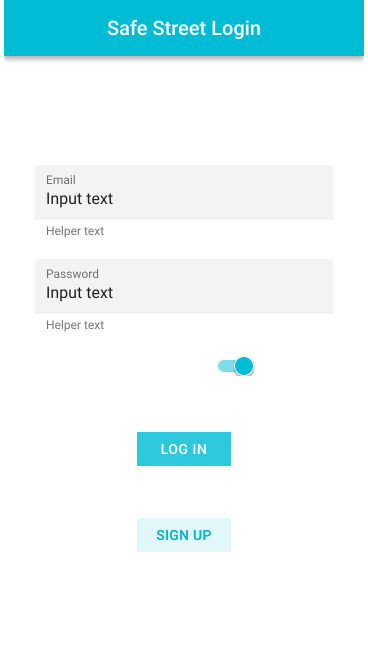
\includegraphics[height=7.7cm,keepaspectratio]{images/mockups/Sign_in.png}
		\caption{Sign-in page}
\end{figure}
\clearpage
\subsubsection{User}
\begin{figure}[!htb]
	\centering
	\begin{minipage}{.45\textwidth}
		\centering
		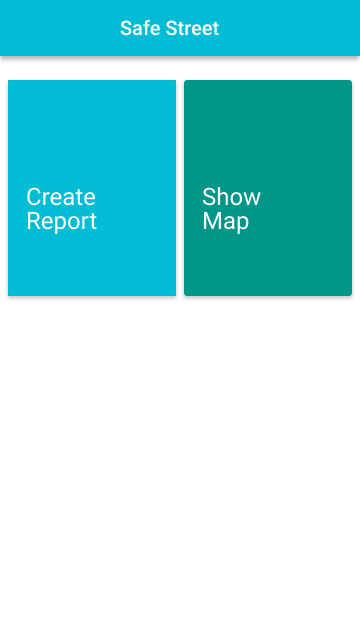
\includegraphics[height=7.7cm,keepaspectratio]{images/mockups/Home_Citizen.png}
		\caption{User HomePage}
	\end{minipage}\quad
	\begin{minipage}{.45\textwidth}
		\centering
		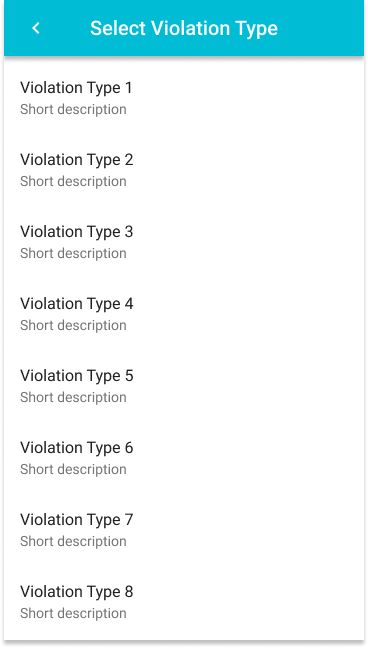
\includegraphics[height=7.7cm,keepaspectratio]{images/mockups/Violation_Type_Menu.png}
		\caption{Select violation type}
	\end{minipage}
\end{figure}

\begin{figure}[!htb]
	\centering
	\begin{minipage}{.45\textwidth}
		\centering
		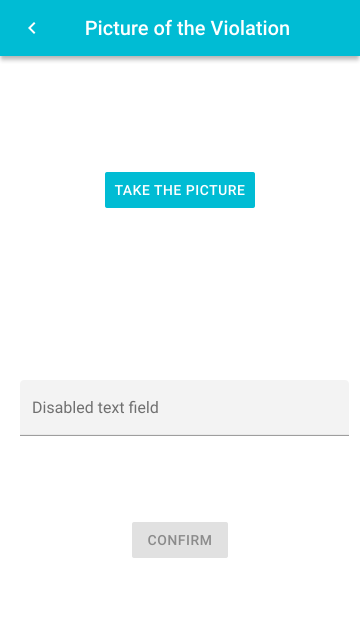
\includegraphics[height=7.7cm,keepaspectratio]{images/mockups/Create_Report_take_picture.png}
		\caption{Take Picture}
	\end{minipage}%
	\begin{minipage}{.45\textwidth}
		\centering
		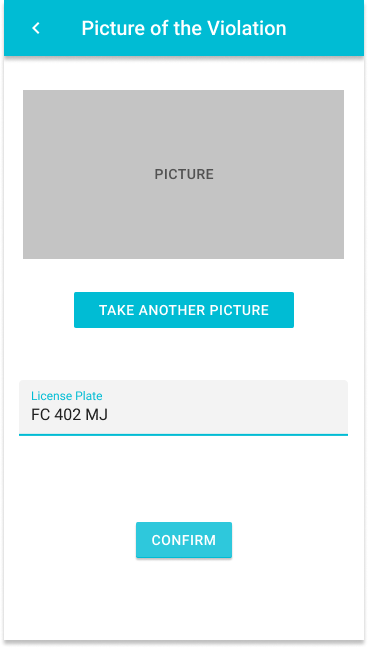
\includegraphics[height=7.7cm,keepaspectratio]{images/mockups/Create_Report_after_picture.png}
		\caption{Check License Plate Number}
	\end{minipage}
\end{figure}

\clearpage
\begin{figure}[!htb]
	\centering
	\begin{minipage}{.45\textwidth}
		\centering
		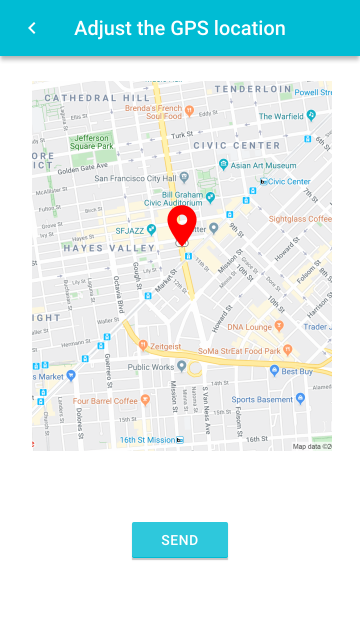
\includegraphics[height=7.7cm,keepaspectratio]{images/mockups/Create_report_GPS.png}
		\caption{Check Location and submit report}
	\end{minipage}\quad
	\begin{minipage}{.45\textwidth}
		\centering
		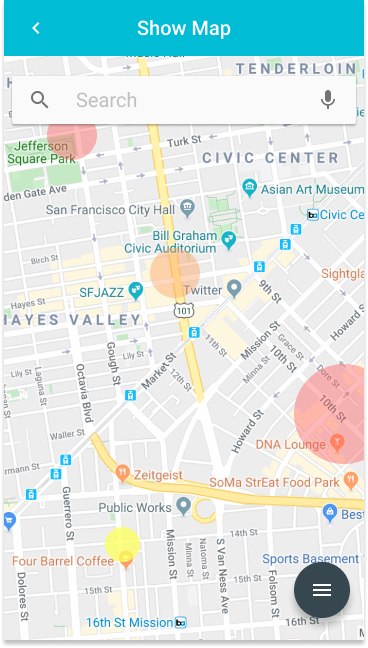
\includegraphics[height=7.7cm,keepaspectratio]{images/mockups/Show_Map.png}
		\caption{Show Map with highlighted area}
	\end{minipage}
\end{figure}

\begin{figure}[!htb]
	\centering
	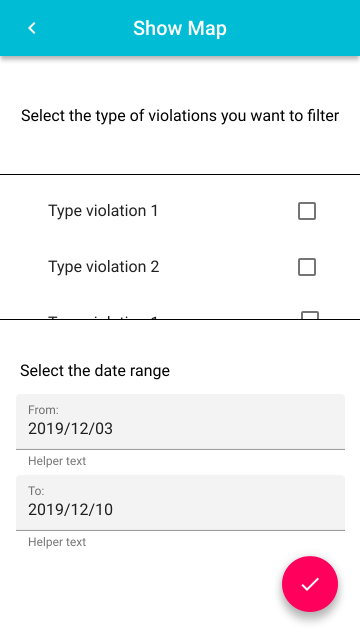
\includegraphics[height=7.7cm,keepaspectratio]{images/mockups/Show_Map_Filter.png}
	\caption{Select data to show on the map}
\end{figure}

\clearpage
\subsubsection{Traffic Warden}
\begin{figure}[!htb]
	\centering
	\begin{minipage}{.45\textwidth}
		\centering
		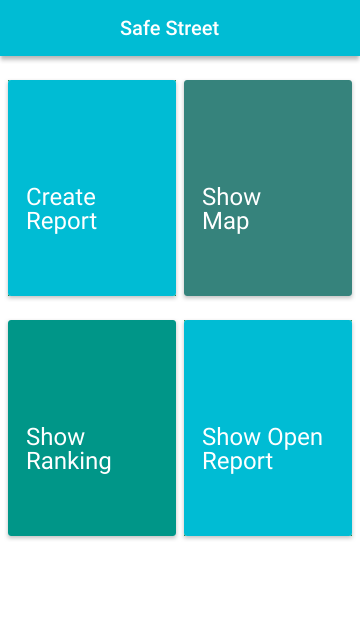
\includegraphics[height=7.7cm,keepaspectratio]{images/mockups/Home_Traffic_Warden.png}
		\caption{Home}
	\end{minipage}%
	\begin{minipage}{.45\textwidth}
		\centering
		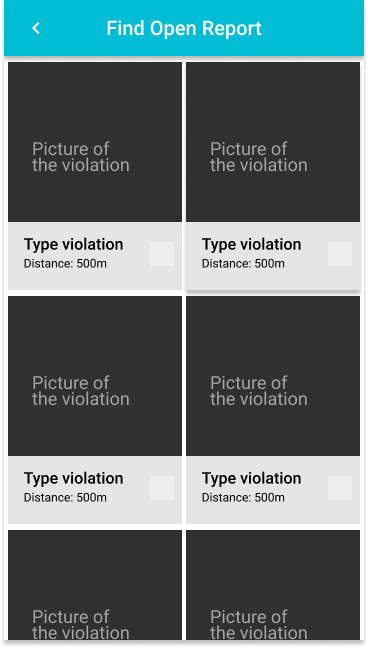
\includegraphics[height=7.7cm,keepaspectratio]{images/mockups/Open_Report_Map.png}
		\caption{Find open report}
	\end{minipage}
\end{figure}

\begin{figure}[!htb]
	\centering
	\begin{minipage}{.45\textwidth}
		\centering
		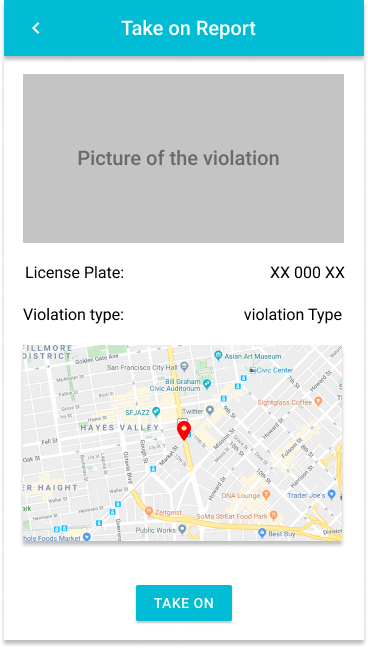
\includegraphics[height=7.7cm,keepaspectratio]{images/mockups/Report_Open_detail.png}
		\caption{Take on report}
	\end{minipage}%
	\begin{minipage}{.45\textwidth}
		\centering
		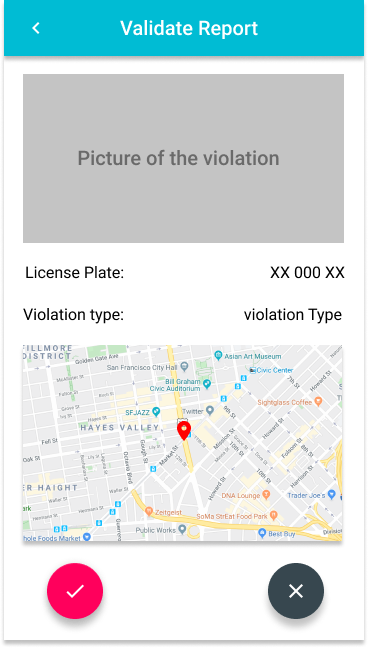
\includegraphics[height=7.7cm,keepaspectratio]{images/mockups/Report_Open_detail_took_on.png}
		\caption{Validate report}
	\end{minipage}
\end{figure}

\begin{figure}[!htb]
	\centering
	\begin{minipage}{.45\textwidth}
		\centering
		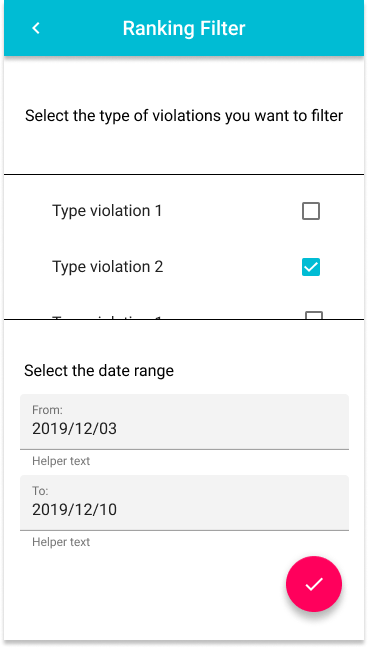
\includegraphics[height=7.7cm,keepaspectratio]{images/mockups/Ranking_Filter.png}
		\caption{Set filter for the Ranking of vehicles}
	\end{minipage}\quad
	\begin{minipage}{.45\textwidth} 
		\centering
		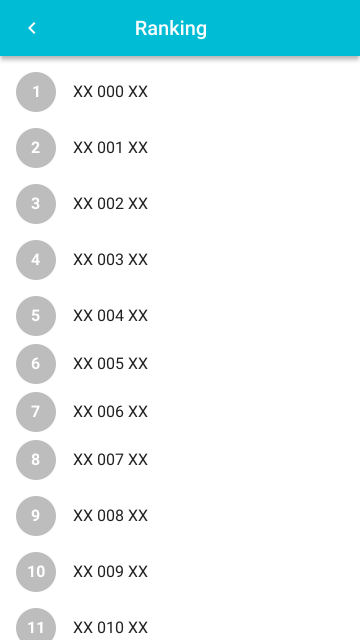
\includegraphics[height=7.7cm,keepaspectratio]{images/mockups/Ranking.png}
		\caption{Check Ranking of vehicles}
	\end{minipage}
\end{figure}

\clearpage
\subsubsection{Municipality's clerk}
\begin{figure}[!htb]
	\centering
	\begin{minipage}{.45\textwidth}
		\centering
		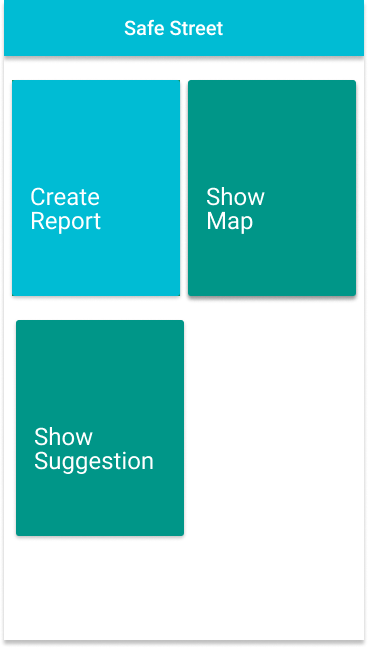
\includegraphics[height=7.7cm,keepaspectratio]{images/mockups/Home_Municipality.png}
		\caption{Home}
	\end{minipage}\quad
	\begin{minipage}{.45\textwidth} 
		\centering
		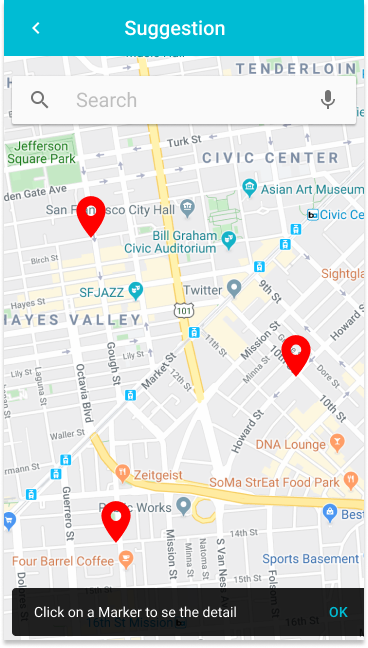
\includegraphics[height=7.7cm,keepaspectratio]{images/mockups/Suggestions.png}
		\caption{Check suggestions}
	\end{minipage}
\end{figure}

\begin{figure}[!htb]
		\centering
		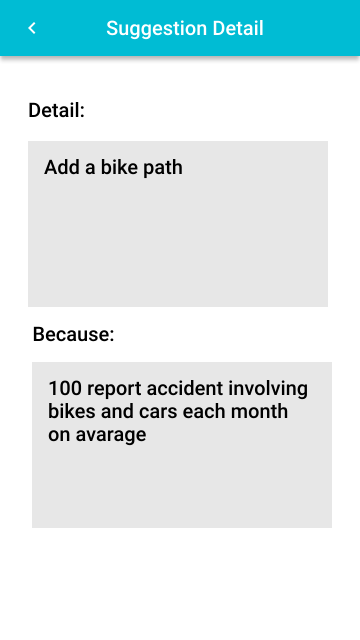
\includegraphics[height=7.7cm,keepaspectratio]{images/mockups/Suggestions_Detail.png}
		\caption{Check suggestion details}
\end{figure}


\clearpage
\subsection{UX Diagrams}
In all the diagrams the actions to go back are omitted to simplify the diagrams.
\begin{itemize} 
	\item \bf User
		\begin{figure}[!htb]
			\centering
			\includegraphics[width=1.0\textwidth]{images/UX/UX-citizen-v2.png}
			\caption{User UX diagram}
		\end{figure}

	\item \bf Traffic warden
		\begin{figure}[!htb]
			\centering
			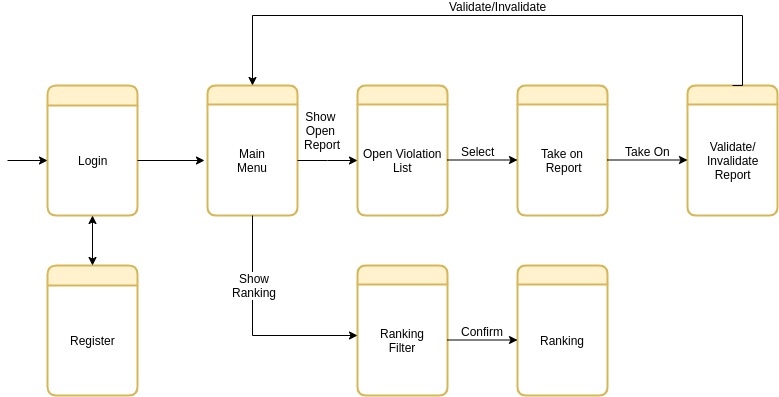
\includegraphics[width=1.0\textwidth]{images/UX/UX-traffic-warden-v2.png}
			\caption{Traffic warden UX diagram}
		\end{figure}
\newpage
	\item \bf Municipality's clerk
		\begin{figure}[!htb]
			\centering
			\includegraphics[width=1.0\textwidth]{images/UX/UX-municipality-v2.png}
			\caption{Municipality's clerk UX diagram}
		\end{figure}
\end{itemize} 

\newpage
\section{Requirements traceability}
The following requirements were described in the RASD:
\begin{itemize}
\item	\textbf{R1} The system has to allow sign up of new users.
\item	\textbf{R2} The system has to allow users to login.
\item	\textbf{R3} The system must allow users to send pictures of violations, including their date, time, and position to authorities.
\item	\textbf{R4} The system, when it receives a picture, must run an algorithm to read the license plate.
\item	\textbf{R5} The system must allow the user to fix the license plate if the algorithm read it wrong.
\item	\textbf{R6} The system must allow the user to fix the location if the GPS acquired the wrong location.
\item	\textbf{R7} The system must store the information of the report sent by the users.
\item	\textbf{R8} The system must send a notification to the traffic warden.
\item	\textbf{R9} The system has to allow one traffic warden to "take on" the report.
\item	\textbf{R10} The system has to allow the traffic warden to validate or to invalidate the report.
\item	\textbf{R11} The system must mine the reports to higlight the streets (or the areas) with the highest frequency of violations.
\item	\textbf{R12} The system has to allow search for a specific location and select from a menu which kind of data he wants to see.
\item	\textbf{R13} The system must distinguish privilege of account (normal, traffic warden, municipality clerk).
\item	\textbf{R14} The system must mine the reports to create a ranking of the vehicles that commit more violation.
\item	\textbf{R15} The system must gather data about accidents from the municipality.
\item	\textbf{R16} The system must cross the information provided by the municipality about the accidents with its own data to identify potentially unsafe areas.
\item	\textbf{R17} The system must show possible interventions to improve unsafe area.
\end{itemize}

Here it's explained how the requirements defined in the RASD map to the components defined in the previous sections.\\
\begin{tabular}{r|l}
\hline
\bf Requirement & \bf Components\\
\hline
	R1 & Authenticator \\& DBMS \\& ClientAPP \\& Router\\ 
\hline
	R1 & Authenticator \\& DBMS \\& ClientAPP \\& Router\\ 
\hline
	R3 & ReportManager \\& ClientAPP \\& Router\\
\hline
	R4 & ReportManager \\& ALPR\\& ClientAPP\\
\hline
	R5 & ClientAPP \\
\hline
	R6 & ClientAPP \\
\hline
	R7 & ReportManager \\& DBMS\\
\hline
	R8 & Firebase \\& NotificationManager \\&  DBMS\\
\hline
	R9 & ReportManager \\& DBMS \\
\hline
	R10 & ReportManager \\& DBMS \\ 
\hline
	R11 & AreaHighlighter \\&ReportManager\\&  DBMS \\
\hline
	R12 & ClientApp \\& Map Provider\\
\hline
	R13 & Authenticator \\& DBMS\\
\hline
	R14 & RankingManager \\&ReportManager\\& DBMS \\
\hline
	R15 & MunicipalityAPI \\&  SuggestionMiner\\
\hline
	R16 & MunicipalityAPI \\&  SuggestionMiner\\& ReportManager \\& DBMS \\
\hline
	R17 & SuggestionDisplayer \\
\hline
\end{tabular}

\clearpage
\section{Implementation, integration and test plan}
\label{sec:ittp}
An accurate analysis of the RASD and DD must be done before starting the implementation of the system.\\
The system is divided in the following subsystems which can be implemented independently one from each other:
\begin{itemize}
	\item Client Applications (Android, iOS, webapp)
	\item Application Server
	\item Web Server
	\item DBMS
	\item External components:
	\begin{itemize}
		\item Map Provider
		\item ALPR
		\item Firebase
		\item MuncipalityAPI
	\end{itemize}
\end{itemize}
The idea is to adopt a bottom-up approach for the implementation strategy, but also, in order to provide first at least the key features of the system, the parts needed by those features will have an high priority.
The table below lists the importance and implementation difficulty of the main features of the system which it is helpful to better understand the implementation and integration plans.
\\ \\
\begin{tabular}{c|c|c}
\hline
\bf Feature & \bf Importance & \bf Implementation \\& \bf for customers & \bf Difficulty\\
\hline
\hline
Sign up and Login & Low & Easy\\
\hline
Report violations & High & Medium \\
\hline
Get notifications & Medium & Easy\\
\hline
Take on reports & High & Medium \\
\hline
Cross data to suggest interventions  & Medium & Hard\\
\hline
Show ranking of vehicles & Low & Easy\\
\hline
Show critical areas & Medium & Medium\\
\hline
Show suggestions & Medium & Medium\\
\hline
\end{tabular}
\\ \\ \\
The table shows how the priority is to have users sending reports and traffic wardens to take on them, which is the  main goal of the system.
The functionalities that allow users to visualize data should pretty easy to provide as they consist in getting data from the database with simple queries and visualize it (as a plain list or on a map).
A more challenging task is to provide an algorithm that can elaborate proper suggestions for possible interventions, however this is an advanced function that does not affect normal users. 

\subsection{Integration Process}
As already stated, the integration will be performed from following a bottom-up approach.
The modules which are being integrated should pass the unit tests in order to be sure that the components are working fine on
their own and that if an integration test fails, the problem is regarding the integration itself.

\subsubsection{Integration Order}
		\begin{figure}[!htb]
			\centering
			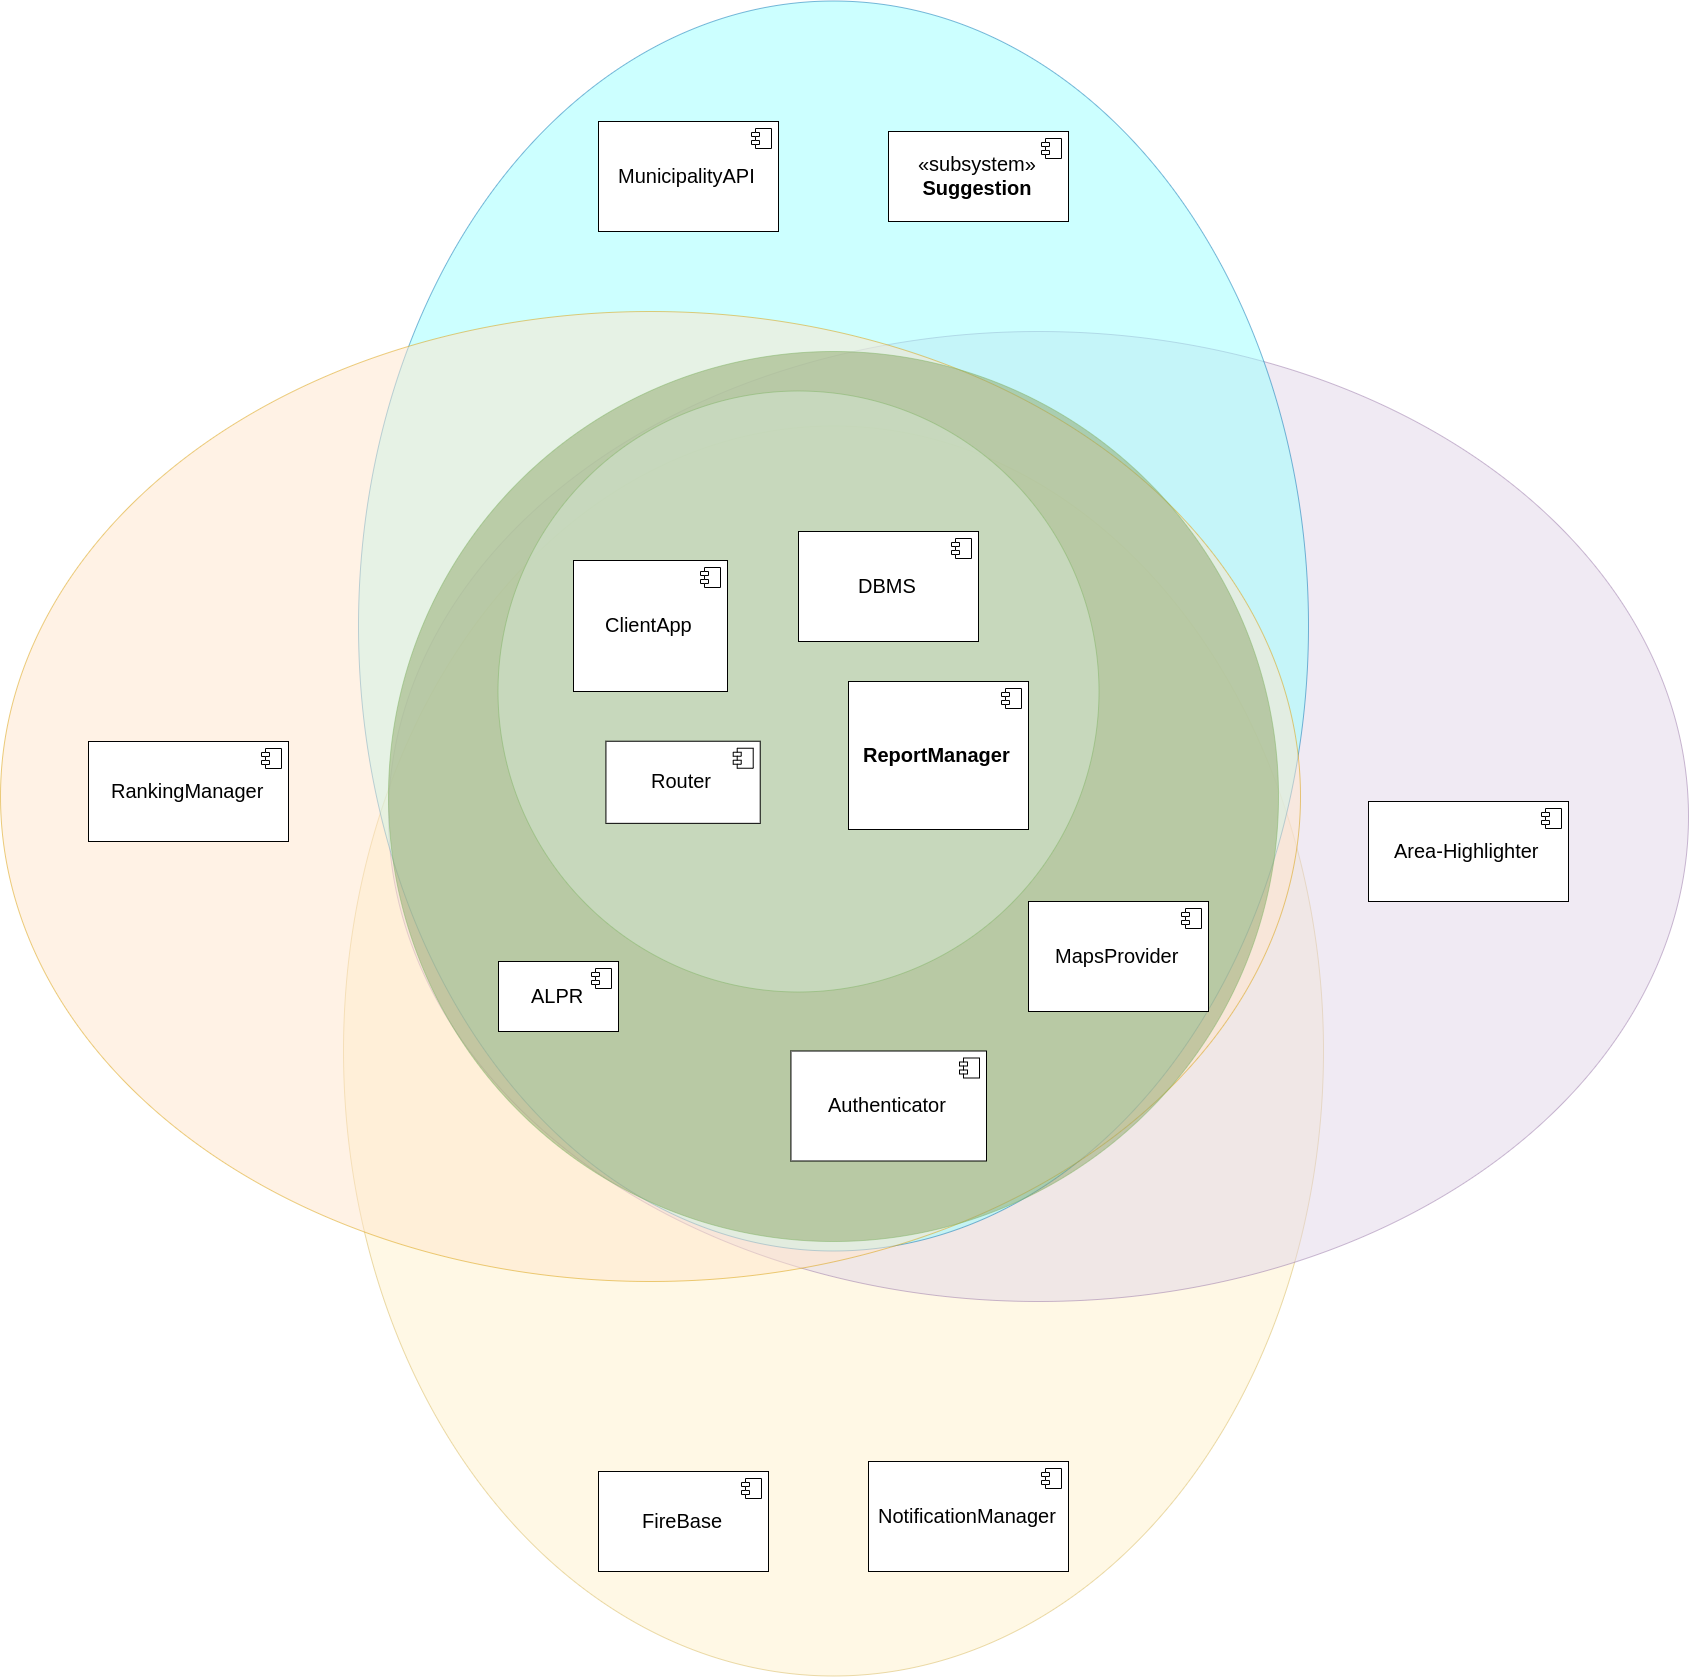
\includegraphics[width=1.0\textwidth]{images/component-integration.png}
			\caption{Integration Order Diagram}
		\end{figure}
\begin{enumerate}
	\item 	The priority is to have the main functionality working ASAP, so the integration between the key components (ClientAPP, Router, ReportManager and DBMS) must be done first. 
		This will be helpful to test the core of the main functionality. 
	\item 	However to actually make it usable in a real use case for an user also the ALPR, MapProvider and Authenticator must be integrated.
	\item 	The NotificationManager and FireBase will then be integrated. 
	\item   The component needed to visualize the critical areas (Area-Highlighter) will be integrated.
	\item   The component needed to elaborate the ranking of vehicles (RankingManager) will be integrated.
	\item   Eventually the components needed to provide the suggestions ( MunicipalityAPI and the Suggestion Subsystem ) will be integrated.
\end{enumerate}
This is the best strategy from the point of view of the standard users.
Which could be a reasonable strategy to adopt because the project is crow-funded.
However, as cleary visible in the diagram, the phases 3,4,5,6 can be switched. 

\subsection{Testing}
A Continuous integration (CI) service like Travis will be used. This service runs tests automatically when pushing code changes providing instant feedback on the code changes. Integrated with proper settings on github it also avoids the merge of code that doesn't pass tests to the master/production branch.
\subsubsection{Unit testing}
Significant unit tests should be written for each component. We don't suggest to adopt a test driven development approach, however appropiate unit tests give several benefits.
(For instance: make it easier to identify bugs in code earlier, simplify debugging process, provide documentation, reduce the time needed to fix bugs.)\\
\textbf{Mocha} (a simple and easy to use JS test framework running on Node.js) will be used for unit testing the application server components.\\
Unit test for the ClientAPP  (developed with Flutter) will be written using the packages suggested by the official documentation: the test package, which provides the core framework for writing unit tests and the fluttertest package, which provides additional utilities.\\
It's important to remind tha unit tests only test individual software components and methods. They don't test databases, network resources, render to screen, or the receive of user actions from outside the process running the test.
Infact also other type of testing are needed.

\subsubsection{Integration testing}
The main goal of integration process is to avoid as much errors as possible at each step of the process. 
The system will incrementally integrate components as soon as they are completely developed and released.
The Bottom-up strategy will be adopted for most of the integration process. In this way we can obtain feedbacks about system
functionalities as soon as components are released and it's possible to parallelize integration of different parts of the system.\\
The router component (which will be an express.js router) will be tested using Mocha and Supertest. 
Supertest is a library written to test HTTP calls in Node.js, which is perfect to write tests for RESTful API.

\subsubsection{Other types of testing}
Once the system is completely integrated, also non-functional requirements should be tested.
For example with security, load, performance and stress testing. \\
The security of the system may be tested, for instance, by doing some penetration tests.

\newpage
\section{Effort spent}
	\begin{center}
		{\bf Cazzola Federico \href{https://github.com/f-cazzola}{@f-cazzola} }
		\vspace{2mm}

			\begin{tabular}{p{1.3cm}|p{1.8cm}|p{6.7cm}}
				\hline
				\bf Date & \bf \makebox[1.8cm][c]{Hours} & \bf \makebox[6.7cm][c]{Description} \\
				23/11/19 & \makebox[1.8cm][c]{2} & \makebox[6.7cm][c]{Architectural design}\\
				24/11/19 & \makebox[1.8cm][c]{3} & \makebox[6.7cm][c]{Architectural design}\\
				29/11/19 & \makebox[1.8cm][c]{2} & \makebox[6.7cm][c]{Architectural design}\\
				30/11/19 & \makebox[1.8cm][c]{6} & \makebox[6.7cm][c]{Architectural design}\\
				01/12/19 & \makebox[1.8cm][c]{8} & \makebox[6.7cm][c]{Architectural design}\\
				04/12/19 & \makebox[1.8cm][c]{4} & \makebox[6.7cm][c]{UI design}\\
				05/12/19 & \makebox[1.8cm][c]{6} & \makebox[6.7cm][c]{UI design and UX}\\
				06/12/19 & \makebox[1.8cm][c]{4.3} & \makebox[6.7cm][c]{UI design and UX}\\
				07/12/19 & \makebox[1.8cm][c]{8} & \makebox[6.7cm][c]{Interfaces, General improvements}\\
				\hline
				total    & \makebox[1.8cm][c]{43.3}
			\end{tabular}
	\end{center}
	\vspace{1cm}

	\begin{center}
		{\bf Dotti Francesco \href{https://github.com/dottif}{@dottif} }
		\vspace{2mm}

			\begin{tabular}{p{1.3cm}|p{1.8cm}|p{6.7cm}}
				\hline
				\bf Date & \bf \makebox[1.8cm][c]{Hours} & \bf \makebox[6.7cm][c]{Description} \\
				\hline
				15/11/19 & \makebox[1.8cm][c]{1} & \makebox[6.7cm][c]{Initial Structure}\\
				22/11/19 & \makebox[1.8cm][c]{1.5} & \makebox[6.7cm][c]{Introduction}\\
				23/11/19 & \makebox[1.8cm][c]{1.5} & \makebox[6.7cm][c]{Architectural design}\\
				29/11/19 & \makebox[1.8cm][c]{0.5} & \makebox[6.7cm][c]{Component view}\\
				30/11/19 & \makebox[1.8cm][c]{6.5}\makebox[6.7cm][c]{Component Deployment Runtime view}\\
				01/12/19 & \makebox[1.8cm][c]{8} & \makebox[6.7cm][c]{Architectural design}\\
				03/12/19 & \makebox[1.8cm][c]{0.5} & \makebox[6.7cm][c]{Architectural design}\\
				04/12/19 & \makebox[1.8cm][c]{2.5} & \makebox[6.7cm][c]{Architectural design}\\
				05/12/19 & \makebox[1.8cm][c]{4} & \makebox[6.7cm][c]{Req. traceability and Implementation}\\
				06/12/19 & \makebox[1.8cm][c]{3} & \makebox[6.7cm][c]{Implementation and Testing}\\
				07/12/19 & \makebox[1.8cm][c]{8} & \makebox[6.7cm][c]{IT,UI, General improvements}\\
				\hline
				total    & \makebox[1.8cm][c]{37}
			\end{tabular}
	\end{center}
\newpage
\section{References}
\begin{itemize}
	\item \href{https://flutter.dev/}{Flutter}
	\item \href{https://firebase.google.com/}{Firebase}
	\item \href{https://www.openalpr.com/}{ALPR}
	\item \href{https://www.mysql.com/}{MySQL}
	\item \href{https://expressjs.com/}{Express.js}
	\item \href{https://nodejs.org/en/}{Node.js}
	\item \href{https://www.npmjs.com/package/supertest}{Supertest}
	\item \href{https://mochajs.org/}{Mocha}
\end{itemize}
\subsection{Software used}
\begin{itemize}
	\item \href{https://www.figma.com/}{Figma}: UI mockups
	\item \href{https://www.draw.io/}{Draw.io}: Diagrams
	\item \href{https://www.latex-project.org/}{LaTeX}: Document preparation system 
	\item \href{https://www.vim.org/}{VIM}: The best Text Editor
	\item \href{https://github.com/xuhdev/vim-latex-live-preview}{Latex plugin for VIM}
	\item \href{https://code.visualstudio.com/}{vs code}: Text Editor with user-friendly live share plugin
\end{itemize} 

\end{document}
